\documentclass[acmsmall,screen,review]{acmart}

% ACM TOMS submission version. The arXiv/preprint version lives in main.tex
% (standard article class, per the redistribution rules for publisher classes).
% Body text is kept identical to main.tex; only the class, front matter, and
% ACM-required metadata differ.

\usepackage{booktabs}
\graphicspath{{figure/}}

\newcommand{\amgcl}{\textsc{amgcl}}
\newcommand{\hypre}{\textsc{hypre}}

%% ACM bibliographic / rights boilerplate (placeholders until acceptance)
\setcopyright{acmlicensed}
\acmJournal{TOMS}
\acmYear{2026}
\acmVolume{0}
\acmNumber{0}
\acmArticle{0}
\acmMonth{1}
\acmDOI{}

\begin{document}

\title{How much is there to gain from tuning an algebraic multigrid solver?}
\subtitle{A cross-library empirical study with cheap, honestly-priced matrix
features}

\author{Chun-Yeol You}
\affiliation{%
  \institution{Department of Physics and Chemistry, DGIST
  (Daegu Gyeongbuk Institute of Science and Technology)}
  \city{Daegu}
  \postcode{42988}
  \country{Republic of Korea}}
\email{cyyou@dgist.ac.kr}

\renewcommand{\shortauthors}{C.-Y. You}

\begin{abstract}
Algebraic multigrid (AMG) is the workhorse preconditioner for large sparse
linear systems, yet its performance depends strongly on internal parameters
--- coarsening scheme, smoother, and strength-of-connection threshold --- that
most users leave at their defaults. We ask two questions empirically. First,
how much speed is left on the table by not tuning these \emph{internal} knobs
(as opposed to the coarser ``which solver'' choice studied previously)? Second,
can a good configuration be predicted from features that are cheap to compute
relative to the solve itself? Sweeping 88 parameter configurations over 150
matrices from the SuiteSparse collection with \amgcl{} (13{,}200 solves), we
find a median oracle speedup of $2.4\times$ over the default (interquartile top
$6.4\times$, maximum $292\times$), with the best configuration varying across
14 distinct coarsening/smoother labels --- so per-matrix selection, not a
single better default, is required. A gradient-boosted predictor trained and
evaluated with a strict leave-one-group-out protocol picks a configuration that
solves $83\%$ of held-out matrices and captures $\sim\!43\%$ of the achievable
speedup, and near-free structural features alone are as good as adding
expensive spectral features that cost $100$--$1000\times$ more. Crucially, we
cross-validate on \hypre{} BoomerAMG and find that while tunability replicates
qualitatively (median oracle $1.6\times$), its magnitude does not transfer
between libraries (rank correlation $0.24$) and is largely governed by default
quality: the dramatic \amgcl{} speedups occur precisely where its default is
weak and \hypre{}'s well-engineered default already wins. Intrinsic solvability,
by contrast, is library-independent (hard-matrix Jaccard $0.76$). All code, the
sweep dataset, and the feature extractor are released for reproduction.
\end{abstract}

\begin{CCSXML}
<ccs2012>
<concept>
<concept_id>10010147.10010257.10010293</concept_id>
<concept_desc>Computing methodologies~Machine learning approaches</concept_desc>
<concept_significance>300</concept_significance>
</concept>
<concept>
<concept_id>10002950.10003714.10003716.10011136</concept_id>
<concept_desc>Mathematics of computing~Solvers</concept_desc>
<concept_significance>500</concept_significance>
</concept>
<concept>
<concept_id>10002950.10003714.10003715.10003736</concept_id>
<concept_desc>Mathematics of computing~Mathematical software performance</concept_desc>
<concept_significance>500</concept_significance>
</concept>
</ccs2012>
\end{CCSXML}

\ccsdesc[500]{Mathematics of computing~Solvers}
\ccsdesc[500]{Mathematics of computing~Mathematical software performance}
\ccsdesc[300]{Computing methodologies~Machine learning approaches}

\keywords{algebraic multigrid, preconditioner, parameter tuning, algorithm
selection, sparse linear solvers, benchmarking, reproducibility}

\maketitle

\section{Introduction}
\label{sec:intro}

Simulations across science and engineering reduce, at their core, to solving
large sparse linear systems $Ax=b$ with millions of unknowns. Algebraic
multigrid (AMG)~\cite{ruge1987,stuben2001,vanek1996} is among the most
effective preconditioners for such systems and is embedded in every major
solver framework~\cite{petsc,trilinos,hypre,amgcl}. Its efficiency, however,
hinges on a handful of internal parameters: the coarsening scheme that builds
the multigrid hierarchy, the smoother that damps error on each level, and the
strength-of-connection threshold that decides which couplings are ``strong.''
These knobs interact, are problem-dependent, and are difficult to set a priori
--- so in practice they are left at library defaults that are rarely optimal.

A substantial literature studies \emph{algorithm selection} for linear
solvers~\cite{rice1976,bhowmick2009,sood2019,tang2022}, but almost all of it
operates at the level of ``which solver / which preconditioner,'' treating an
entire AMG method as a single categorical label. The interior of that label ---
the coarsening $\times$ smoother $\times$ threshold space that this paper
targets --- is comparatively unexplored, even though library documentation
itself admits the defaults are problem-dependent. Two further methodological
gaps recur. Feature-based selection studies seldom charge the cost of computing
their features against the speedup those features buy; and predictor evaluation
typically uses random cross-validation, which leaks sibling matrices from the
same problem family across the train/test split and inflates reported accuracy.

This work is a systematic, AI-assisted empirical study in the spirit of recent
performance-engineering case studies~\cite{you2026mumax,you2026qiskit}: we hold
the measurement discipline fixed and vary only what we intend to measure. We
make four contributions.
\begin{enumerate}
\item We quantify the oracle speedup available from tuning \emph{internal} AMG
parameters over 150 SuiteSparse matrices and 88 \amgcl{} configurations, and
show it is large and requires per-matrix selection
(Section~\ref{sec:tuning}).
\item We build a predictor from features tiered by cost, evaluate it with a
strict leave-one-group-out protocol, and show that near-free structural
features suffice --- expensive spectral features add nothing despite costing
$100$--$1000\times$ more (Section~\ref{sec:predictor}).
\item We cross-validate on a second, independent AMG library (\hypre{}
BoomerAMG) and show that tunability replicates qualitatively but its magnitude
is library-dependent and driven by default quality, whereas intrinsic
solvability is library-independent (Section~\ref{sec:crosslib}).
\item We release all tooling and the full sweep dataset for reproduction.
\end{enumerate}

\section{Related work}
\label{sec:related}

The algorithm-selection problem dates to Rice~\cite{rice1976}; general surveys
are given by Kotthoff~\cite{kotthoff2016}. For sparse linear solvers,
Bhowmick et al.~\cite{bhowmick2009} framed solver selection as classification
with feature-computation cost as an explicit concern. The most comprehensive
study is Sood's~\cite{sood2019}, which labelled over 1{,}000 SuiteSparse
matrices against $154$ PETSc solver--preconditioner configurations and found
that a small set of inexpensive matrix features nearly matches the full set.
More recent work applies graph neural networks: Tang, Zhang and
Chen~\cite{tang2022} predict one of 33 PETSc solver+preconditioner classes,
and a parallel line learns preconditioners directly~\cite{chen2024gnp,
hausner2025}. All of these choose \emph{among} methods or configurations at a
coarse granularity; none systematically tunes the interior parameters of a
single AMG method, which is our focus.

On the AMG side, the classical Ruge--St\"uben method~\cite{ruge1987} and
smoothed aggregation~\cite{vanek1996} define the coarsening families we sweep;
BoomerAMG~\cite{henson2002,hypre} and its parallel coarsening
schemes~\cite{desterck2006} provide the second library for cross-validation,
and \amgcl{}~\cite{amgcl} the first. We use the SuiteSparse Matrix
Collection~\cite{davis2011} as the matrix source and Krylov
methods~\cite{hestenes1952,saad1986,vandervorst1992,saad2003} as accelerators.

\section{Methodology}
\label{sec:method}

\paragraph{Matrices.}
We draw 150 real, square matrices from the SuiteSparse
collection~\cite{davis2011} with $10^4 \le n \le 5\times10^5$ and at least
three nonzeros per row on average, deliberately selecting \emph{multiple}
matrices from each of 43 problem groups so that a leave-one-group-out
evaluation has within-family structure to generalise across. Pure
graph/network collections, on which AMG is not expected to work, are excluded.

\paragraph{Parameter grid.}
For \amgcl{} we cross three coarsening schemes (smoothed aggregation,
plain aggregation, Ruge--St\"uben) with four strength-threshold values, eight
relaxation schemes (\texttt{spai0/1}, damped Jacobi, Gauss--Seidel, Chebyshev,
ILU(0), ILU(k) for $k\in\{1,2\}$), giving 88 configurations per matrix. SPD
matrices are solved with conjugate gradients, others with BiCGStab. The
strength-threshold path differs between coarsening families and is handled
per-family.

\paragraph{Measurement discipline.}
Every configuration is timed as setup${}+{}$solve to a relative residual of
$10^{-8}$, with a right-hand side $b = A x^\ast$ for a fixed ramp
$x^\ast_i = 1 + i/n$; the all-ones vector, used in a pilot, is degenerate for
zero-row-sum matrices ($b=0$) and was discarded. Each solve is repeated in
process and the minimum reported, since scheduler noise can only add time. To
avoid memory-bandwidth contention corrupting timings, we run one
single-threaded solver process per compute node and distribute matrices across
nodes; a contention probe confirmed that co-running even four solves inflates a
$36$~ms solve to $116$~ms. Runs are capped at 30~s wall-clock; failures are
recorded by type (diverged, stalled at max-iterations, timed out, errored).
Experiments ran on the DGIST iREMB cluster.

\paragraph{Features and predictor.}
We extract features in three cost tiers: Tier~0 (structure: size, density,
row-nonzero distribution, bandwidth, pattern symmetry, diagonal presence),
Tier~1 (cheap value-based: diagonal dominance, value asymmetry, a
Gershgorin bound, a few power-iteration steps), and Tier~2 (a sparse
condition-number estimate). The predictor is a gradient-boosted
classifier/regressor~\cite{friedman2001,scikit} that, given matrix features and
a one-hot configuration encoding, predicts whether a configuration will
succeed and its log solve-time; per matrix it picks the fastest
predicted-successful configuration. \textbf{All predictor numbers use
leave-one-group-out cross-validation}: every matrix from a held-out SuiteSparse
group is excluded from training, so no sibling leaks across the split.

\section{How much is there to gain from tuning?}
\label{sec:tuning}

Figure~\ref{fig:oracle} shows the per-matrix \emph{oracle speedup}, the ratio
of the default configuration's time to the best configuration's time, over the
41 matrices where both solved. The median is $2.4\times$, the upper quartile
exceeds $6.4\times$, and the maximum reaches $292\times$; $21$ of $41$ matrices
gain at least $2\times$. Beyond speed, tuning changes feasibility: on 31
matrices the default configuration fails outright while some configuration
succeeds. Tuning is therefore not a marginal optimisation but often the
difference between solving and not solving.

\begin{figure}[t]
\centering
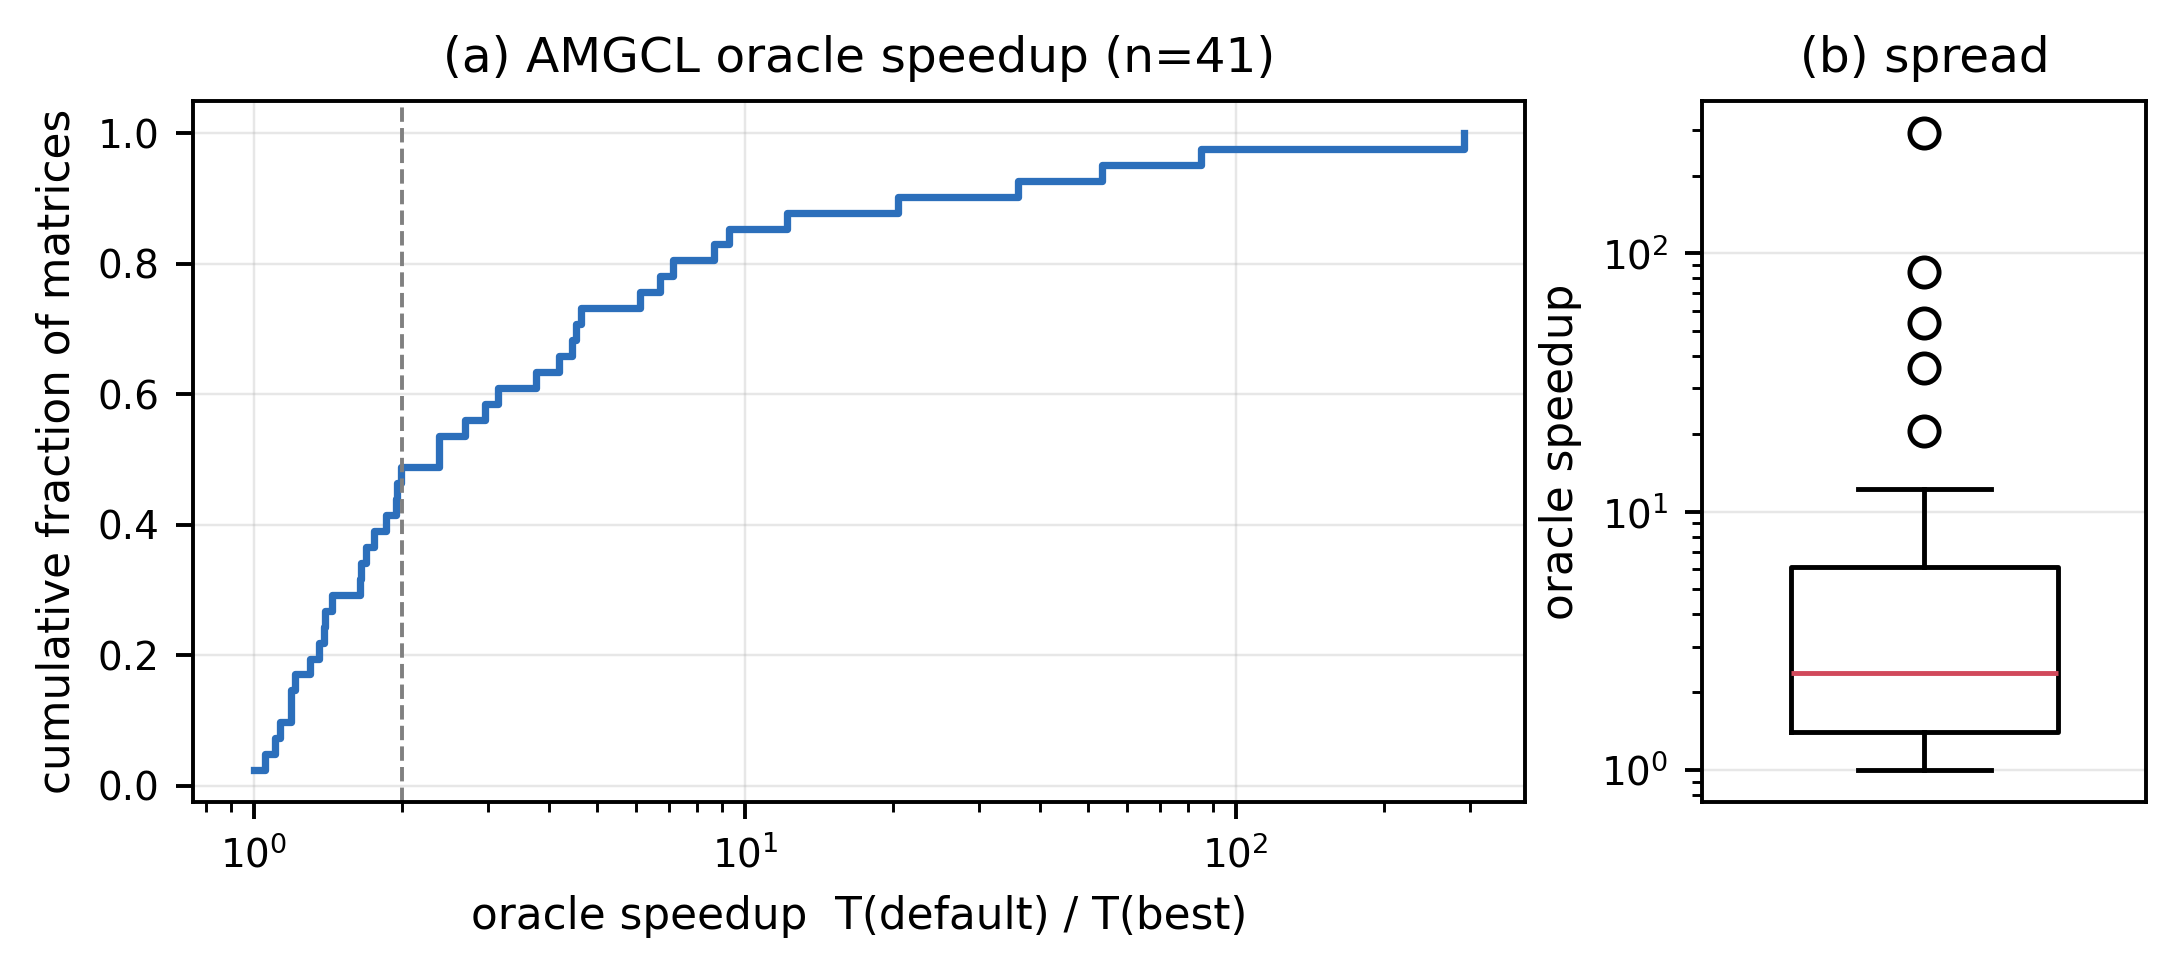
\includegraphics[width=\textwidth]{fig_oracle_dist.png}
\caption{\amgcl{} oracle speedup over 41 matrices: (a) empirical CDF (log axis;
dashed line at $2\times$), (b) distribution on a log scale. Median $2.4\times$,
upper quartile $6.4\times$, maximum $292\times$.}
\label{fig:oracle}
\end{figure}

Critically, no single configuration dominates. Figure~\ref{fig:winners} counts
how often each coarsening/relaxation label is the per-matrix winner: 14
distinct labels win across the matrices, and the \amgcl{} default
(smoothed aggregation with \texttt{spai0}) is almost never among them. There is
thus no ``just change the default'' fix; capturing the available speedup
requires choosing per matrix.

\begin{figure}[t]
\centering
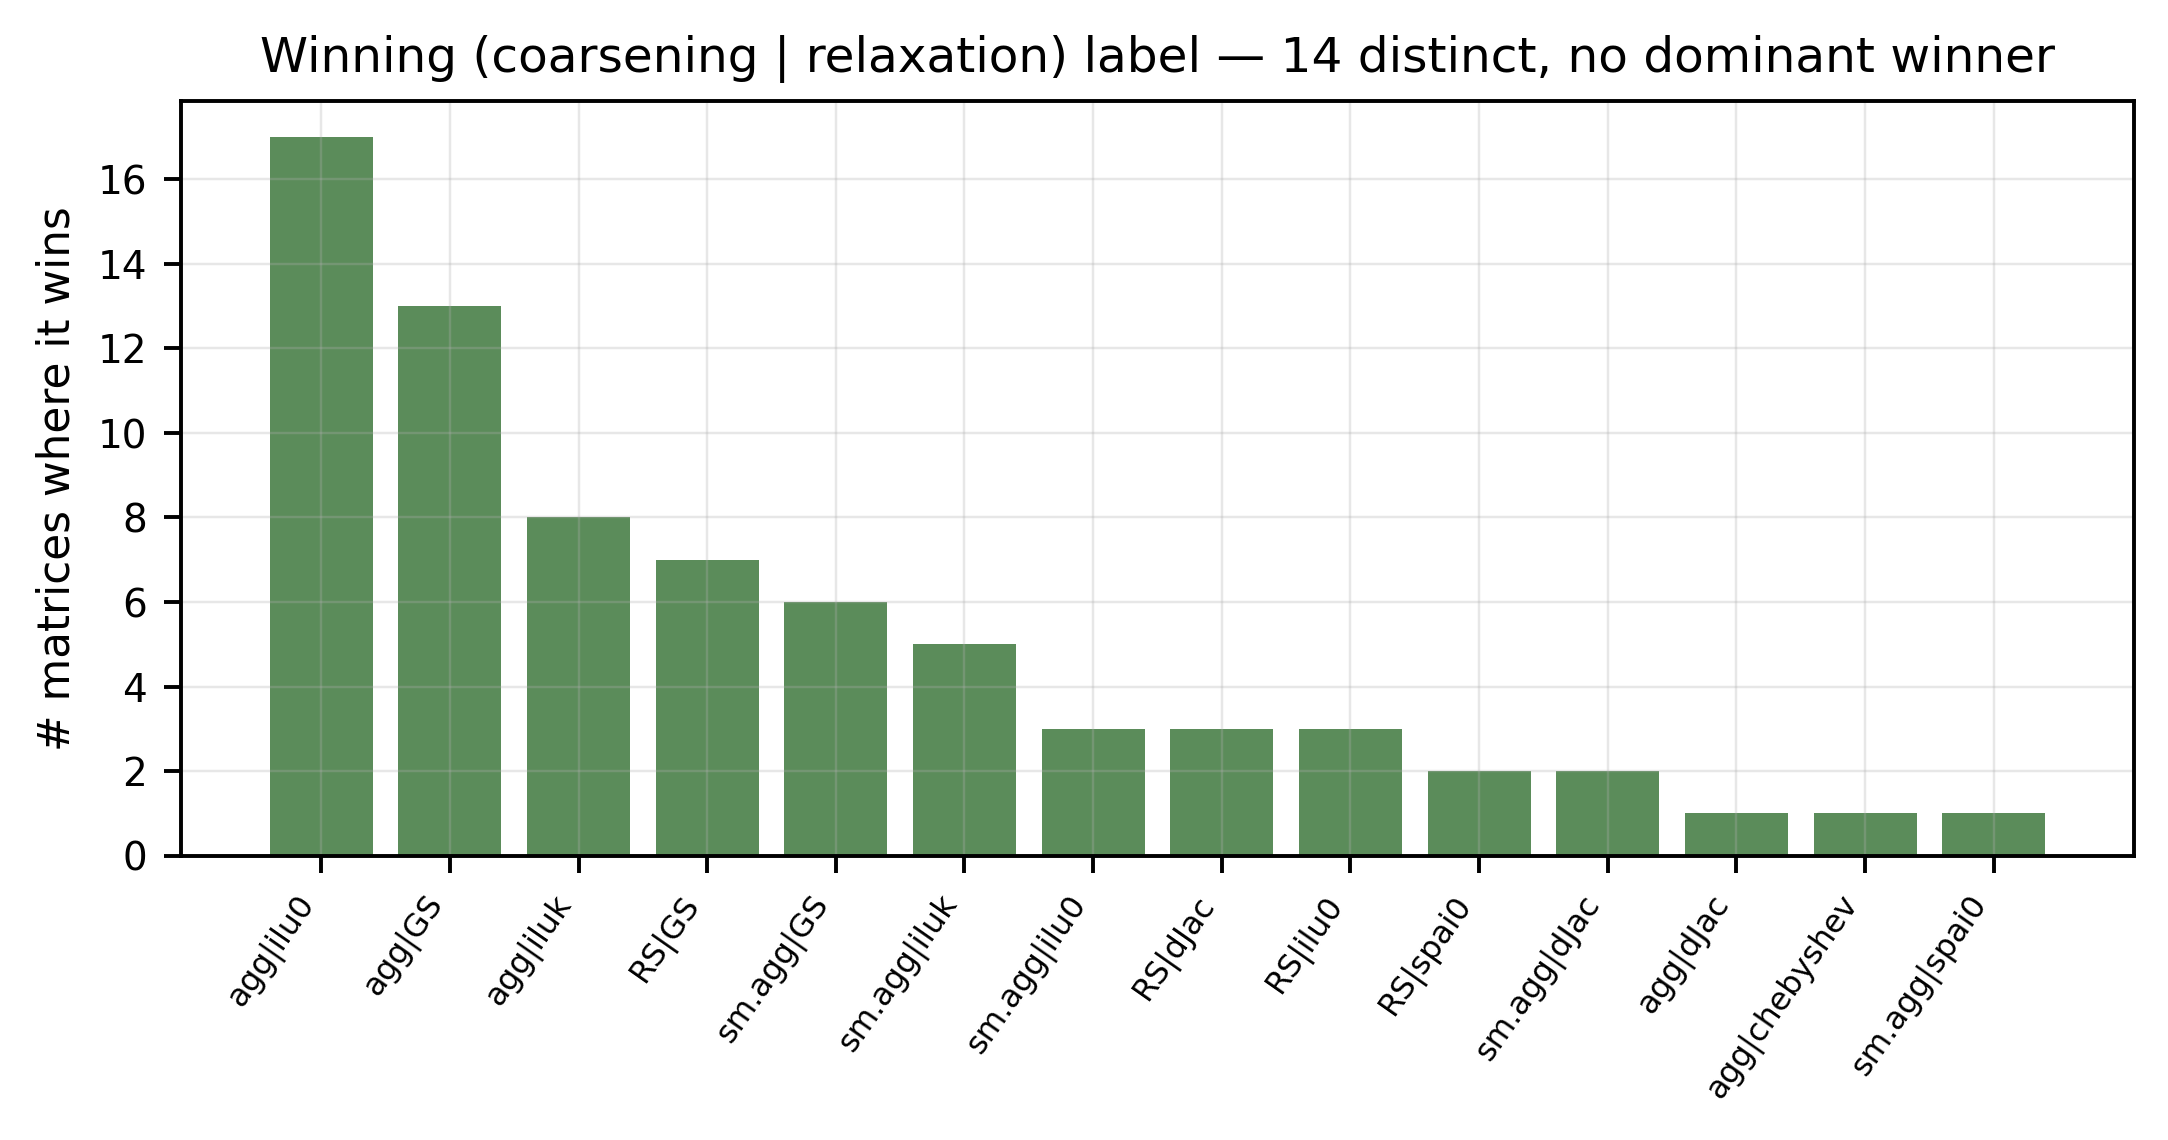
\includegraphics[width=\textwidth]{fig_winners.png}
\caption{Frequency with which each (coarsening $\vert$ relaxation) label is the
per-matrix winner. The spread across 14 labels shows that per-matrix selection,
not a single improved default, is what the speedup requires.}
\label{fig:winners}
\end{figure}

\section{Predicting a good configuration cheaply}
\label{sec:predictor}

Can the winning region be predicted without solving? Under leave-one-group-out
evaluation, a per-(matrix, configuration) success classifier reaches accuracy
$0.84$ against a majority baseline of $0.76$. Used end-to-end --- picking one
configuration per held-out matrix --- the predictor selects a configuration
that actually solves $83\%$ of the time and captures a median $43\%$ of the
oracle speedup (Figure~\ref{fig:predictor}), i.e.\ roughly a $1.45\times$
median speedup over the default from features alone, while also steering away
from the defaults that fail.

The most practically useful finding concerns feature cost. Tier~2 spectral
features cost $100$--$1000\times$ more than Tier~0/1 (Figure~\ref{fig:cost}:
median Tier~0 $28$~ms, Tier~1 $+44$~ms, Tier~2 $+8.8$~s per matrix, and the
condition-number estimate frequently fails to converge). Yet adding Tier~1 to
Tier~0 does not improve the predictor ($43\%\to40\%$ captured), and Tier~2 is
unusable at scale. Near-free structural features are sufficient. This directly
addresses the feature-cost gap in prior work: for this task, the expensive
features are not worth their price.

\begin{figure}[t]
\centering
\begin{minipage}[t]{0.48\textwidth}
\centering
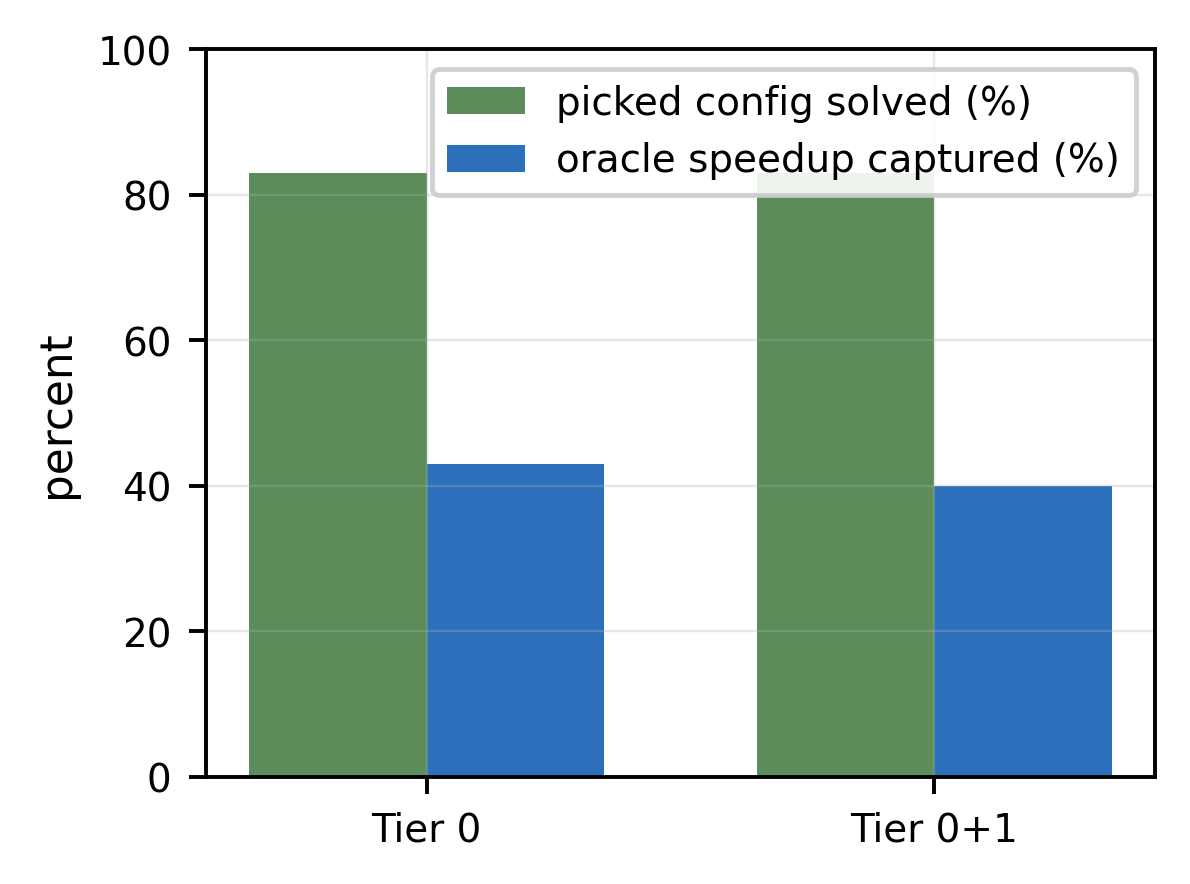
\includegraphics[width=\textwidth]{fig_predictor.png}
\caption{Predictor under leave-one-group-out: fraction of held-out matrices
whose picked configuration solves, and fraction of oracle speedup captured.
Tier~0 (near-free) matches Tier~0+1.}
\label{fig:predictor}
\end{minipage}\hfill
\begin{minipage}[t]{0.48\textwidth}
\centering
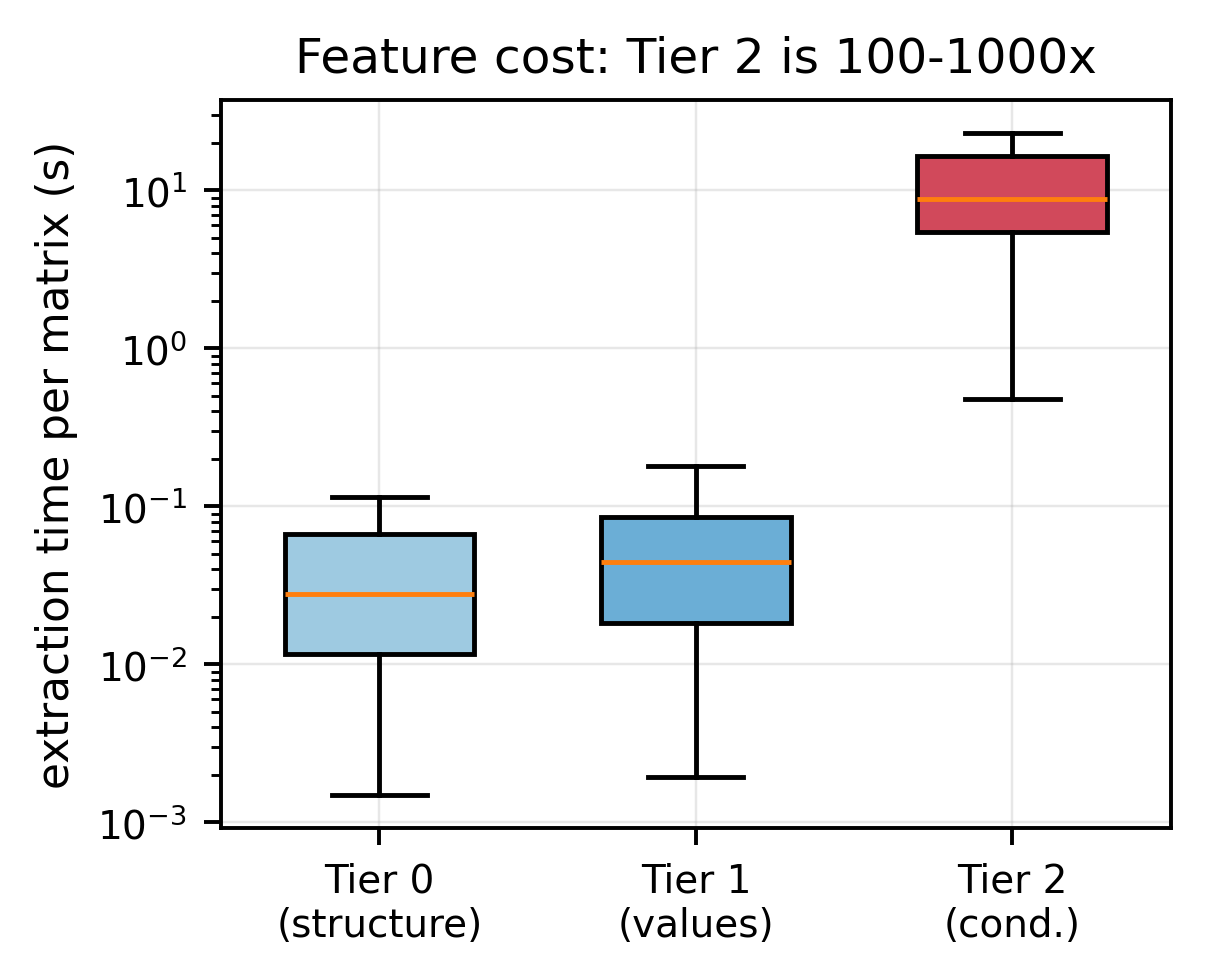
\includegraphics[width=\textwidth]{fig_feature_cost.png}
\caption{Feature-extraction time per matrix by tier (log scale). Tier~2 costs
$100$--$1000\times$ Tier~0/1 yet buys no predictive accuracy here.}
\label{fig:cost}
\end{minipage}
\end{figure}

\paragraph{More data helps.}
To check that the predictor is not saturated by the 150-matrix training set,
we doubled it to 300 matrices (a strict superset, preserving the
multiple-per-group structure) and re-evaluated under the same
leave-one-group-out protocol. The predictor improves rather than plateaus: the
number of evaluable matrices rises from 41 to 66, the picked configuration
solves $89\%$ of held-out matrices (up from $83\%$), and the captured oracle
speedup rises to a median $49\%$ (from $43\%$), while the oracle distribution
itself stays stable (median $2.3\times$, maximum $292\times$). Tier~0 features
remain sufficient at the larger scale ($49\%$ vs.\ $37\%$ for Tier~0+1). More
labelled matrices therefore strengthen the signal, and the near-free feature
finding is not an artifact of the smaller set.

\section{Cross-library validation: does this generalise?}
\label{sec:crosslib}

Are these findings specific to \amgcl{}, or a property of AMG? We repeat the
sweep on \hypre{} BoomerAMG~\cite{henson2002} --- an independent,
widely-deployed library --- over the same 150 matrices, with a matched 36-point
grid (Falgout/PMIS/HMIS coarsening $\times$ four smoothers $\times$ three
thresholds) and identical measurement discipline.

\paragraph{Tunability replicates, but modestly.}
\hypre{} also exhibits a per-matrix oracle speedup (median $1.6\times$, upper
quartile $2.1\times$, maximum $31\times$; 16 default-fails-tuned-succeeds
matrices; 22 distinct winners). So ``internal parameters matter'' holds
qualitatively in both libraries --- but the magnitude is smaller in \hypre{}.

\paragraph{Magnitude is default-driven, not intrinsic.}
Figure~\ref{fig:crosslib} plots per-matrix oracle speedups of the two libraries
against each other: the rank correlation is only $0.24$. A matrix that is very
tunable in \amgcl{} is not necessarily tunable in \hypre{}. Comparing the two
libraries' \emph{defaults} head-to-head explains why: \hypre{}'s default is
faster on 26 of 36 shared matrices (median $0.70\times$ the \amgcl{}-default
time) and solves nine matrices the \amgcl{} default fails. Moreover, every one
of the ten highest-\amgcl{}-oracle matrices (including the $292\times$ case) is
one where \hypre{}'s default already beats \amgcl{}'s default. The dramatic
\amgcl{} speedups are therefore largely a \emph{weak-default artifact}: they
measure how far \amgcl{}'s default is from optimal on those matrices, not an
intrinsic, library-independent tuning headroom.

\paragraph{Intrinsic difficulty is library-independent.}
By contrast, the set of matrices that no configuration solves overlaps strongly
between libraries (Jaccard $0.76$). Whether a problem is solvable by AMG at all
is a property of the matrix; how much tuning helps is a property of the
matrix--library pair.

\paragraph{A predictor confirms both directions.}
The same predictor approach applies to \hypre{}: under leave-one-group-out it
picks a configuration that solves $87\%$ of held-out matrices and captures a
median $47\%$ of \hypre{}'s (modest) oracle --- comparable to the \amgcl{}
figures. More tellingly, transferring \emph{matrix-level} models across
libraries reproduces the two-part story. A ``will any configuration solve this
matrix?'' classifier trained on one library and tested on the other beats its
majority baseline by $+0.25$ to $+0.33$: intrinsic solvability transfers. But a
regressor for the per-matrix oracle magnitude, trained on one library and
tested on the other, predicts the target with rank correlation only
$\approx\!0.2$: tuning benefit does not transfer. Difficulty is a
library-independent property of the matrix; tunability is not.

\begin{figure}[t]
\centering
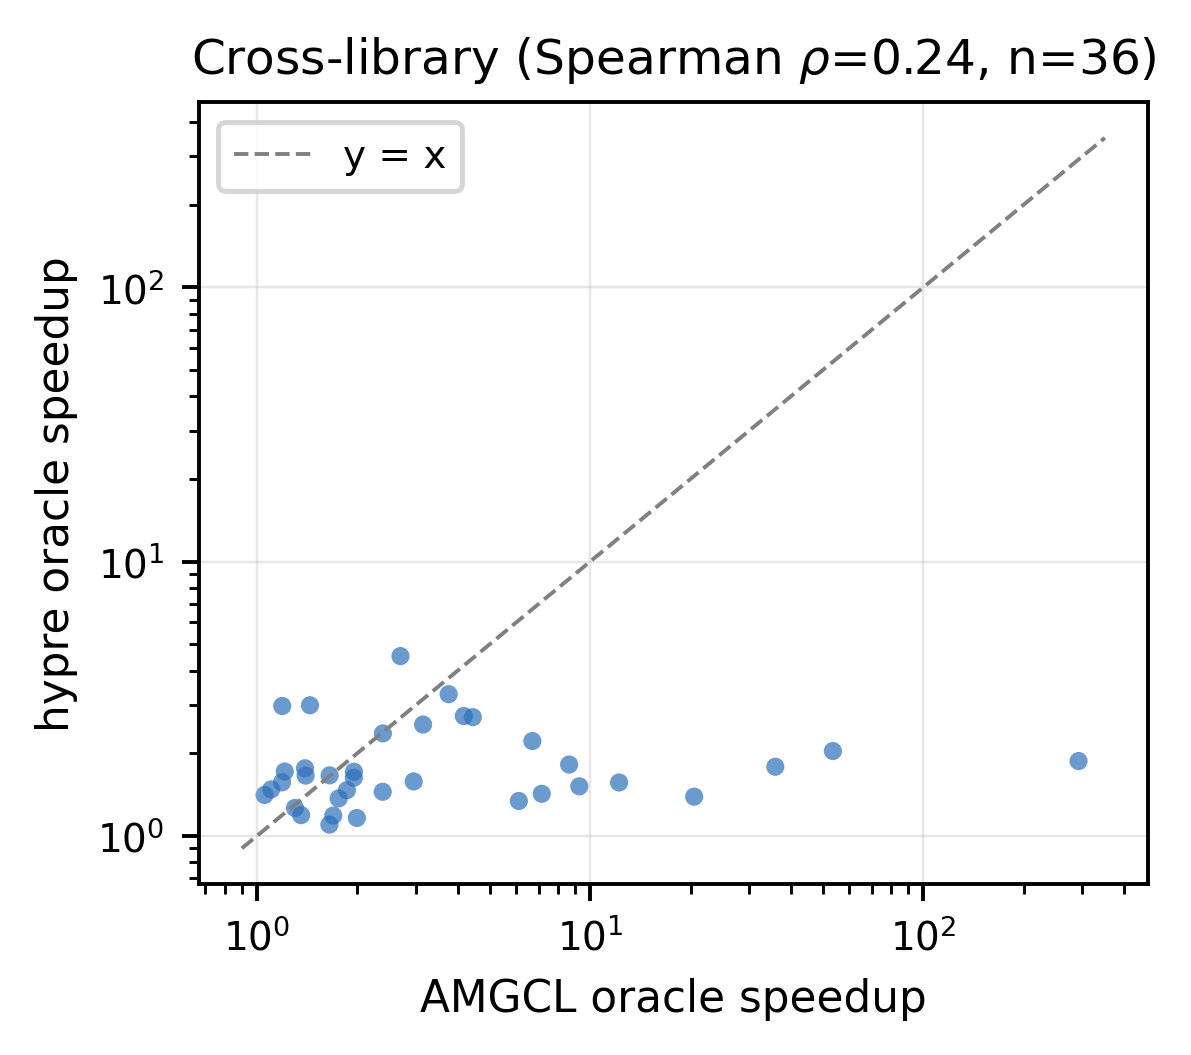
\includegraphics[width=0.6\textwidth]{fig_crosslib.png}
\caption{Per-matrix oracle speedup: \amgcl{} vs \hypre{} (both log axes,
$n=36$). The weak rank correlation ($\rho=0.24$) shows tuning benefit does not
transfer between libraries; the largest \amgcl{} gains are where \hypre{}'s
default already wins.}
\label{fig:crosslib}
\end{figure}

\section{Discussion}
\label{sec:discussion}

The picture that emerges is more nuanced than ``tuning gives large speedups.''
Internal AMG parameter tuning yields real gains in both standard libraries, but
their size is governed largely by how good the library's default already is,
and does not transfer between libraries. This has a clear practical
implication: automatic parameter selection is most valuable for libraries or
regimes with weaker defaults, and its value should be reported \emph{relative
to a strong baseline} to avoid overstating it --- a caveat our own \amgcl{}
figures make concrete. At the same time, that a near-free feature set predicts
useful configurations under an honest group-wise split is encouraging for
building lightweight, always-on auto-tuning into solver libraries.

\paragraph{Limitations.}
The predictor captures $\sim\!43\%$ of the oracle, not all of it; the study
covers 150 matrices and two CPU AMG libraries; and cross-library absolute-time
comparisons are confounded by implementation differences and are read only as
trends. Extending to more matrices, to distributed/GPU backends, and to a
\hypre{}-native predictor with cross-library transfer are natural next steps.

\section{Conclusion}
\label{sec:conclusion}

Tuning the internal parameters of algebraic multigrid --- not merely choosing
among solvers --- offers a median $2.4\times$ and occasionally
order-of-magnitude speedup in \amgcl{}, requires per-matrix selection, and can
be partly predicted from features that cost essentially nothing, with expensive
spectral features adding no value. Cross-validation on \hypre{} BoomerAMG shows
the phenomenon is real but its magnitude is default-dependent and
non-transferable, while intrinsic solvability is library-independent. We
release all code and data so these claims can be reproduced and extended.

\begin{acks}
This work was supported by the National Research Foundation of Korea (NRF)
(No.\ RS-2026-25502724) and the Strategic Research Program under the DGIST R\&D
Program (26-SR-01) of the Ministry of Science, ICT, and Future Planning.

\emph{Generative AI disclosure.} In accordance with the ACM Policy on
Authorship, the author discloses the use of an AI coding assistant (Claude
Code, Anthropic) in this work: it assisted in implementing the benchmark
harness, the tiered feature extractor, and the gradient-boosted predictor; in
orchestrating the parameter sweeps and the cross-library build on the compute
cluster; and in drafting and revising this manuscript. All experimental design
decisions, numerical results, and scientific claims were checked by the author
against the released code and data. The AI system is not an author and bears no
responsibility for the content; the author takes full responsibility for all
material herein.
\end{acks}

\bibliographystyle{ACM-Reference-Format}
\begin{thebibliography}{99}

\bibitem{you2026mumax} C.-Y. You. 2026.
Optimization of MuMax3 by using Claude Code: A CUDAgraph-based case study
in AI-assisted performance engineering.
\emph{J. Magn.} 31 (2026), 204.
https://doi.org/10.4283/JMAG.2026.31.2.204

\bibitem{you2026qiskit} C.-Y. You. 2026.
Variance-reduced trajectory unravelings for GPU noisy quantum-circuit
simulation: Characterization and a Qiskit-Aer integration gap.
arXiv:2607.17678 (2026).

\bibitem{ruge1987} J. W. Ruge and K. St\"uben. 1987.
Algebraic multigrid. In \emph{Multigrid Methods}. SIAM, 73--130.

\bibitem{stuben2001} K. St\"uben. 2001.
A review of algebraic multigrid.
\emph{J. Comput. Appl. Math.} 128 (2001), 281--309.

\bibitem{vanek1996} P. Van\v{e}k, J. Mandel, and M. Brezina. 1996.
Algebraic multigrid by smoothed aggregation for second and fourth order
elliptic problems. \emph{Computing} 56 (1996), 179--196.

\bibitem{brandt1985} A. Brandt, S. F. McCormick, and J. Ruge. 1985.
Algebraic multigrid (AMG) for sparse matrix equations. In \emph{Sparsity and
Its Applications}. Cambridge University Press.

\bibitem{xu2017} J. Xu and L. Zikatanov. 2017.
Algebraic multigrid methods. \emph{Acta Numerica} 26 (2017), 591--721.

\bibitem{henson2002} V. E. Henson and U. M. Yang. 2002.
BoomerAMG: A parallel algebraic multigrid solver and preconditioner.
\emph{Appl. Numer. Math.} 41 (2002), 155--177.

\bibitem{hypre} R. D. Falgout and U. M. Yang. 2002.
hypre: A library of high performance preconditioners. In \emph{Computational
Science -- ICCS 2002} (LNCS 2331). Springer, 632--641.

\bibitem{desterck2006} H. De Sterck, U. M. Yang, and J. J. Heys. 2006.
Reducing complexity in parallel algebraic multigrid preconditioners.
\emph{SIAM J. Matrix Anal. Appl.} 27 (2006), 1019--1039.

\bibitem{amgcl} D. Demidov. 2019.
AMGCL: An efficient, flexible, and extensible algebraic multigrid
implementation. \emph{Lobachevskii J. Math.} 40 (2019), 535--546.

\bibitem{petsc} S. Balay et al. 2023.
PETSc/TAO Users Manual. Technical Report ANL-21/39. Argonne National Laboratory.

\bibitem{trilinos} M. A. Heroux et al. 2005.
An overview of the Trilinos project.
\emph{ACM Trans. Math. Softw.} 31 (2005), 397--423.

\bibitem{pyamg} N. Bell, L. N. Olson, and J. Schroder. 2022.
PyAMG: Algebraic multigrid solvers in Python.
\emph{J. Open Source Softw.} 7 (2022), 4142.

\bibitem{davis2011} T. A. Davis and Y. Hu. 2011.
The University of Florida sparse matrix collection.
\emph{ACM Trans. Math. Softw.} 38 (2011), 1:1--1:25.

\bibitem{saad2003} Y. Saad. 2003.
\emph{Iterative Methods for Sparse Linear Systems} (2nd ed.). SIAM.

\bibitem{hestenes1952} M. R. Hestenes and E. Stiefel. 1952.
Methods of conjugate gradients for solving linear systems.
\emph{J. Res. Natl. Bur. Stand.} 49 (1952), 409--436.

\bibitem{saad1986} Y. Saad and M. H. Schultz. 1986.
GMRES: A generalized minimal residual algorithm for solving nonsymmetric
linear systems. \emph{SIAM J. Sci. Stat. Comput.} 7 (1986), 856--869.

\bibitem{vandervorst1992} H. A. van der Vorst. 1992.
Bi-CGSTAB: A fast and smoothly converging variant of Bi-CG for the solution of
nonsymmetric linear systems.
\emph{SIAM J. Sci. Stat. Comput.} 13 (1992), 631--644.

\bibitem{trefethen1997} L. N. Trefethen and D. Bau. 1997.
\emph{Numerical Linear Algebra}. SIAM.

\bibitem{george1973} A. George. 1973.
Nested dissection of a regular finite element mesh.
\emph{SIAM J. Numer. Anal.} 10 (1973), 345--363.

\bibitem{rice1976} J. R. Rice. 1976.
The algorithm selection problem. \emph{Adv. Comput.} 15 (1976), 65--118.

\bibitem{kotthoff2016} L. Kotthoff. 2016.
Algorithm selection for combinatorial search problems: A survey. In \emph{Data
Mining and Constraint Programming} (LNCS 10101). Springer, 149--190.

\bibitem{bhowmick2009} S. Bhowmick, B. Toth, and P. Raghavan. 2009.
Towards low-cost, high-accuracy classifiers for linear solver selection. In
\emph{Computational Science -- ICCS 2009} (LNCS 5544). Springer, 463--472.

\bibitem{sood2019} K. Sood. 2019.
\emph{Iterative Solver Selection Techniques for Sparse Linear Systems}.
Ph.D. Dissertation. University of Oregon.

\bibitem{eijkhout2010} V. Eijkhout and E. Fuentes. 2010.
Machine learning for multi-stage selection of numerical methods. In \emph{New
Advances in Machine Learning}. InTech.

\bibitem{tang2022} Z. Tang, H. Zhang, and J. Chen. 2022.
Graph neural networks for selection of preconditioners and iterative solvers.
In \emph{NeurIPS 2022 Workshop (GLFrontiers)}.

\bibitem{chen2024gnp} J. Chen. 2024.
Graph neural preconditioners for iterative solutions of sparse linear systems.
arXiv:2406.00809 (2024).

\bibitem{hausner2025} P. H\"ausner, O. \"Oktem, and J. Sj\"olund. 2025.
Neural incomplete factorization: Learning preconditioners for the conjugate
gradient method. In \emph{Northern Lights Deep Learning Conference (NLDL)}.

\bibitem{trifonov2024} V. Trifonov et al. 2024.
Learning from linear algebra: A graph neural network approach to preconditioner
design for conjugate gradient solvers. arXiv:2405.15557 (2024).

\bibitem{friedman2001} J. H. Friedman. 2001.
Greedy function approximation: A gradient boosting machine.
\emph{Ann. Statist.} 29 (2001), 1189--1232.

\bibitem{scikit} F. Pedregosa et al. 2011.
Scikit-learn: Machine learning in Python.
\emph{J. Mach. Learn. Res.} 12 (2011), 2825--2830.

\bibitem{falgout2006} R. D. Falgout, J. E. Jones, and U. M. Yang. 2006.
The design and implementation of hypre, a library of parallel high performance
preconditioners. In \emph{Numerical Solution of PDEs on Parallel Computers}.
Springer, 267--294.

\end{thebibliography}

\end{document}
